\documentclass{elsarticle}


\usepackage{graphicx, subfigure}        % standard LaTeX graphics tool
                             % when including figure files
\usepackage{url}
\usepackage{fixme}
\usepackage{lscape}

\journal{Journal of Artificial Intelligence}

%%%%%%%%%%%%%%%%%%%%%%%%%%%%%%%%%%%%%%%%%%%%%%%%%%%%%%%%%%%%%%%%%%%%%%%%%%%%%%%%%%%%%%%%%

%% Custom macros
\newcommand{\stmt}[1]{{\footnotesize $\langle$\stmttt#1\relax$\rangle$}}
\newcommand{\rawstmt}[1]{{\footnotesize \stmttt#1\relax}}
\def\stmttt#1 #2 #3\relax{{\tt#1} {\bf{\tt #2}} {\tt #3}}

\newcommand{\setstmt}[1]{{\footnotesize [\setstmttt#1\relax]}}
\def\setstmttt#1,#2\relax{\rawstmt{#1}, \rawstmt{#2}}

\newcommand{\concept}[1]{{\footnotesize \texttt{#1}}}

\newcommand{\ie}{{\textit{i.e.~}}}
\newcommand{\cf}{{\textit{cf~}}}
\newcommand{\eg}{{\textit{e.g.~}}}

%%%%%%%%%%%%%%%%%%%%%%%%%%%%%%%%%%%%%%%%%%%%%%%%%%%%%%%%%%%%%%%%%%%%%%%%%%%%%%%%%%%%%%%%%

\begin{document}
\begin{frontmatter}

\title{When the robot considers the human... }
% Use \titlerunning{Short Title} for an abbreviated version of
% your contribution title if the original one is too long
\author{Rachid Alami, Mathieu Warnier, Julien Guitton, S\'{e}verin Lemaignan and Emrah Akin Sisbot}
% Use \authorrunning{Short Title} for an abbreviated version of
% your contribution title if the original one is too long
\address{ LAAS-CNRS\\ 
        Universit\'e de Toulouse, UPS, INSA, INP, ISAE, LAAS\\ 
         F-31077 Toulouse, France\\ \texttt{Firstname.Name@laas.fr}}

\begin{abstract}
  This paper addresses some key decisional issues that are
  necessary for a cognitive robot which shares space and tasks with a
  human. We adopt a constructive approach based on the identification
  and the effective implementation of individual and collaborative
  skills. The system is comprehensive since it aims at dealing with a
  complete set of abilities articulated so that the robot controller
  is effectively able to conduct in a flexible manner a collaborative
  task with a human partner. These abilities include geometric
  reasoning and situation assessment based essentially on
  perspective-taking and affordances, management and exploitation of
  each agent (human and robot) knowledge in a separate cognitive
  model, human-aware task planning and human and robot interleaved
  plan achievement.
\end{abstract}

\begin{keyword}
    %% keywords here, in the form: keyword \sep keyword

    %% MSC codes here, in the form: \MSC code \sep code
    %% or \MSC[2008] code \sep code (2000 is the default)

\end{keyword}

\end{frontmatter}


\section{The challenge of human-robot interaction}

Human-robot interaction requires to equip the robot with explicit
reasoning on the human and on its own capacities to achieve its tasks
in a collaborative way with a human partner. This paper presents a
robot control system which has been especially designed for a
cognitive robot which shares space and task with a human. We have
adopted a constructive approach based on effective individual and
collaborative skills. The system is comprehensive since it aims at
dealing with a complete set of abilities articulated so that the robot
controller is effectively able to conduct in a flexible manner a
collaborative task with a human partner.

We illustrate below how we deal with a typical human-robot interactive
task achievement and what are the abilities we claim are
necessary. Section \S\ref{sec:problem} proposes a typical human-robot
interaction problem that can be solved by the proposed robot
controller. Section \S\ref{sec:soa} reviews related work and analyses
the context of our contribution.  Section \S\ref{sec:Framework}
provides an overview of the robot controller and introduces three
activities which are described in \S\ref{sec:situ}, \S\ref{sec:plan}
and \S\ref{sec:action}. Finally, Section \S\ref{sec:expes} presents an
effective run on a real robot in face to face interaction with a
person.

\subsection{The typical human-robot interaction problem}\label{sec:problem}

Let us consider a robot which is supposed to achieve interactive
object manipulation, fetch and carry tasks and similar tasks in a
domestic environment. The problem we are dealing with here is the
following. Given:
\begin {itemize}
\item a joint goal, which has been previously established and agreed
  upon (through a process which is out of the scope of this paper),
\item the current situation, acquired through perception or
  deduction from previous perceptions, including the state of the
  environment of the robot and of the human,
\end {itemize}
the robot controller computes an action to execute and who (the 
human or the robot, or both in case of a joint action) has to perform
it, and then controls or monitors its execution. The operation
continues until the goal is achieved, is declared unachievable or is
abandoned by the human.

To do so, the robot has to be equipped with a number of decisional, planning
and interpretation abilities where its human partner is taken
explicitly into account. It needs to be able:
\begin {itemize}
\item to build and maintain relevant robot and human beliefs
  (from the robot perspective) with respect to state of the world and the task,
\item to build and maintain iteratively shared (human-robot) plans, 
\item to refine and execute the actions it has to perform, and to monitor 
those achieved by its human partner.
\end {itemize}

Besides, we would like to build such abilities in a generic way, and
to provide several levels of parametrization allowing to adapt to
various environments, and various levels of involvement of the robot
ranging from teammate behavior to assistant or proactive helper.

\subsection{Related work and vision}\label{sec:soa}

The human presence brings new requirements for robot's abilities both
at the functional and at the deliberative levels~\cite{Klein2004}. The
topics involve motion~\cite{Kulic2007,Berg2004,Madhav2006},
navigation~\cite{Althaus2004,Sisbot2007}, manipulation~\cite{Kemp2007}
in presence of humans as well as perception of human
activities~\cite{Breazeal2001,Burger2008}. Also, when
interacting with humans, robots need to incorporate communication and
collaboration abilities. Several theories dealing with
collaboration~\cite{Cohen1991,Grosz1996,Clark1996} emphasize that
collaborative tasks have specific requirements compared to individual
ones, \eg, since the robot and the person share a common goal, they
have to agree on the manner to realize it, they must show their
commitment to the goal during execution, etc. Several robotic systems
have already been built based on these
theories~\cite{Rich1997,Sidner2005,Tambe2005a,Breazeal2003} and they
all have shown benefits of this approach. They have also shown how
difficult it is to manage turn-taking between communication partners
and to interleave task realization and communication in a generic
way. Finally, today only few
systems~\cite{Fong_2006,Breazeal2003,Sisbot2008} take humans into
account at all levels.

Perspective Taking is a human ability which allows one to put
him/herself in another person's point of view. Studied in
psychology literature~\cite{Flavell1992,Tversky1999}, this ability is
crucial when interacting with people by allowing one to reason on
others' understanding of the world in terms of visual perception, spatial
descriptions, affordances and beliefs, etc.
Therefore, in the last years these notions have been gradually
employed in Human-Robot Interaction.~\cite{breazeal2006} presents a
learning algorithm that takes into account information about a
teacher's visual perspective in order to learn a
task. ~\cite{Johnson2005} apply visual perspective taking for action
recognition between two robots.~\cite{Trafton2005} use both visual and
spatial perspective taking for finding out the referent indicated by a
human partner.

Spatial reasoning~\cite{O'Keefe1999}, on the other hand, has been used
for natural language processing for applications such as direction
recognition ~\cite{Kollar2010,Matuszek2010} or language
grounding~\cite{Tellex2010}.~\cite{Skubic2004} presented a spatial
reasoner integrated in a robot which computes symbolic positions of
objects.

\begin{figure}[htb]
\centering
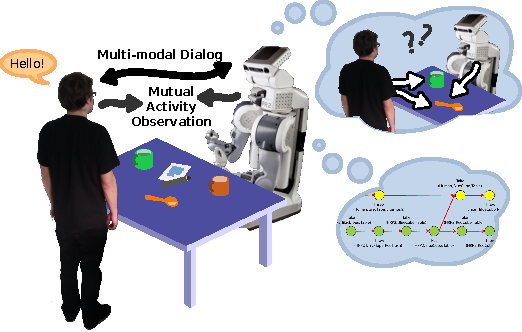
\includegraphics[width=0.9\columnwidth]{figs/grounding_robot.pdf}
\caption{Robot reasoning about HRI and anticipation of human activities:
  sources of information are multi-modal dialogue, and observation of
  environment and human activity}
\label{fig:hri-dec}
\end{figure}

We envision HRI in a context where two agents (a human and a robot)
share a common space and exchange information through various
modalities. Our aim is to endow the robot with an explicit
consideration of the human and with the ability to manage its
interactions with him (Figure~\ref{fig:hri-dec}). This must be
considered at the architecture level as well as at the task/motion
planning and execution level. 

We have devised a decisional framework for human-robot interactive
task achievement that is aimed to allow the robot not only to
accomplish its tasks but also to produce behaviors that support its
engagement vis-a-vis its human partner and to interpret human
behaviors and intentions. 
Together and in coherence with this framework, we have developed
and experimented various task planners and interaction schemes that
allow the robot to select and perform its tasks while taking into
account explicitly the human abilities as well as the constraints
imposed by the presence of humans, their needs and preferences. 

\section{The LAAS deliberative layer}
\label{sec:Framework}

Fig.~\ref{fig|archi} give an overview of the connections between the
deliberative components of our architecture~\cite{Alami2011}.

\begin{figure*}
        \centering
        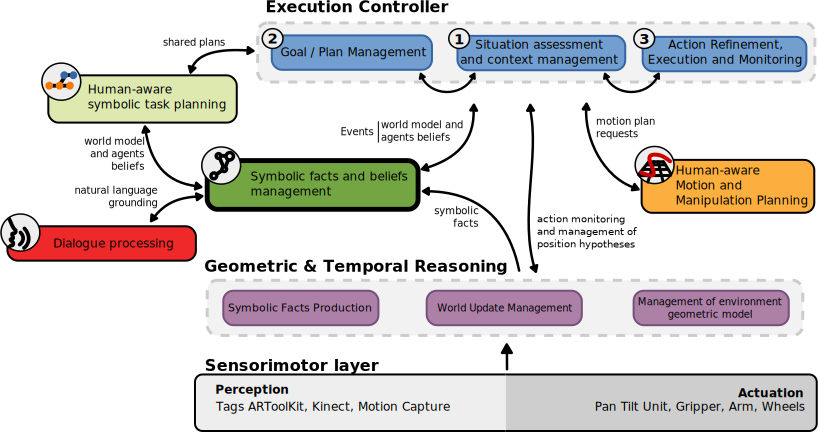
\includegraphics[width=1.0\columnwidth]{figs/archi}
        \caption{Overview of the LAAS deliberative layer. Knowledge is
        centrally managed in an active \emph{semantic blackboard}, pictured
        above with a thick border.}
        \label{fig|archi}
\end{figure*}


This architecture moves away from standard layered approaches. Interactions
between components are mostly bidirectional and, from the software components
point of view, we do not introduce layers of abstraction (we do, however, have
access to the lower level modules of the robot to execute
actions~\cite{Alami1998}, but all cognition-related modules reside at the same
level). This is especially visible for the dialogue input processing. This
component does not simply act as an alternative perceptual input to the
symbolic database, but also actively queries previously acquired knowledge to
disambiguate and validate the newly created symbolic knowledge (see
section~\ref{sect|com}).

Our architecture relates but is to be distinguished from \emph{Beliefs,
Desires, Intentions} (BDI) architectures. BDI architectures are primarily
focused on \emph{practical reasoning}, \ie the process of deciding, step by
step, which action to perform to reach a goal (as summarised by
Woolridge~\cite{Woolridge1999}). The management of the interaction between
knowledge (the beliefs) and task and plan representation and execution (the
desires and the intentions) is central, and aims at selecting at each step the
best subgoal. It becomes then an intention that the robot commits to.

This interaction between knowledge and actions is also central to our approach
(as for any cognitive system), but task representation and task execution is
not seen as a monolithic, central function: it is one of the activities of the
robot, actually split between communication components (that can acquire
desires from interaction with agents, amongst other things) and an execution
controller that may decide to take an incoming desire into account to create
its own internal goals. The controller generates and controls intentions from
these goals with the help of a symbolic task planner, that has also direct
access to the knowledge base.

The architecture is not only focused on this workload, and other
activities are conducted without being explicitly considered as desires:
assessment of the situation and the environment, dialogue (including
performative dialogue that can possibly change the internal state of the robot,
but does not lead to the creation of desires,  like question answering or
statement assertion), various background monitoring and recognition tasks, etc.

Regarding the anchoring question, this architecture is bidirectional. The
components we described provide a \textit{bottom-up} grounding process:
geometric reasoning and dialogue processing modules constantly build and push
new symbolic contents about the world to the knowledge base where it becomes
accessible to decisional layers. In parallel, the knowledge base relies on
reasoning in a \textit{top-down} way to produce new facts that may trigger in
return physical behaviours.

\subsection*{Knowledge model}

In our architecture (Fig.~\ref{fig|archi}), knowledge manipulation relies on a
\emph{semantic blackboard}: one central server (the {\sc Oro}
server~\cite{Lemaignan2010}) stores knowledge as it is produced by each of the
deliberative components. It conversely exposes an API to query the knowledge
base.

Knowledge is represented as RDF triples in the OWL sub-language. Each
time triples are added or removed from the knowledge base, a Description
Logics reasoner ({\sc Pellet}\footnote{\url{http://clarkparsia.com/pellet/}})
classifies the whole ontology and inserts all possible inferred triples.

Relying on RDF triples and Description Logics has major advantages like the
availability of numerous open-source libraries to manipulate the ontology,
interoperability with several major on-line knowledge bases (like {\sc
OpenCyc}, {\sc WordNet} or {\sc DBPedia}), open-world reasoning, and the formal
guarantee of decidability (it is always possible to classify a Description
Logics ontology).

It has also notable limitations: RDF triples imply only binary predicates
(\stmt{subject predicate object}), which constrains the expressiveness of the
system or leads to cumbersome reifications. Alternative exists (like {\sc
KnowRob}~\cite{Tenorth2009a}) that mixes RDF with more expressive logic
languages like {\sc Prolog}, at the price, however, of other limitations, like
closed-world reasoning or immutable T-Box. The classification
performance is another issue: from our experience, with an ontology sized for a
standard experiment (about 100 classes and 200 instances), classification
typically take about 100ms, which becomes problematic during interactions.
Besides, the performances are difficult to predict, since a seemingly
inoffensive new statement may indirectly change radically the logical
complexity of the whole knowledge model and lead to notable degradation of
classification time.

This knowledge model also largely exclude representation of continuous
phenomena (like time) or uncertain phenomena. When required, these have to be
managed by dedicated components.

Amongst the features of {\sc Oro}, the system can dynamically creates
new independent knowledge models (\ie independent instantiations of the
ontology). This feature is used for instance to store separately the beliefs of
each of the agents the robot interacts with (see section~\ref{sect|tom}).

\subsection*{Interaction model}

Interaction happens as a consequence of an explicit request of the
human to satisfy a goal or because the robot finds itself in a
situation where it is useful if not mandatory. In both cases, the
robot has a goal to satisfy.  An important issue is the notion of
engagement, a process in which the robot will have to establish,
maintain and terminate a connection with a human partner. 
This covers goal establishment, selection of an incremental refinement
of the task that is intended to be achieved, and execution control
including monitoring, and even influencing, human task performance and
his/her commitment to the goal. The human involvement may range from a
direct participation to the task achievement, to a simple
``acceptance'' of robot activity in his/her close vicinity.

Next sections describe how the robot is controlled through an analysis of the
three main activities performed by the robot controller:

\begin {enumerate}
\item Situation assessment and context management 
\item Goals and plans management
\item Action refinement, execution and monitoring
\end {enumerate}

These activities are caried out by different software composants:

\begin{itemize}

    \item Situation assessment is managed by \textsc{Spark} (Spatial Reasoning
        and Knowledge module)~\cite{Sisbot2011},

    \item HATP (Human-Aware Task Planner)~\cite{Alili2008} is responsible for
        symbolic task planning,

    \item We finally also rely on a set of human-aware motion, placement and
        manipulation planners, grouped under the \textsc{Move3D}
        umbrella~\cite{Sisbot2008, Mainprice2011, Pandey2010}.

\end{itemize}

Other decisional activities, such as situated dialog (\cite{Ros2010b,
  Lemaignan2011}, not presented here) have been developed that use the
same set of components.

\section{Situation assessment and context management}\label{sec:situ}

This activity involves the geometric and temporal reasoning component,
the symbolic facts and belief management component and the dedicated
robot controller activity (Figure~\ref{architecture_fg}).

We assume that perception provides in real-time the identity and the
position of objects when they are in the field of view of the sensors.
In our implemented examples, the robot is localised using a standard
horizontal laser-scanning based localisation system, the objects are
identified and localized using ARToolkit \cite{ARToolkit} and the
humans are tracked using a commercial motion capture system and a
Kinect device from Microsoft.

\subsection{Geometric and Temporal Reasoning component}\label{sub:gtrc}

The geometric reasoning component plays a central role in our
architecture. It is called SPARK (Spatial Reasoning and
Knowledge~\cite{Sisbot2011}) in the current implementation. It is
responsible for geometric information gathering and it embeds a number
of decisional activities linked to abstraction (symbolic facts
production) and inference based on geometric and temporal reasoning.
SPARK maintains all geometric positions and configurations of agents,
objects and furniture coming from perception and previous or {\it a
  priori} knowledge.

 %\subsubsection*{Symbolic facts production:} 
\vspace{0.3cm}
\noindent
\textbf{Symbolic facts production:} 
Geometric state of the world is abstracted in symbolic facts that can
be classified in three different categories.

\begin {itemize}
\item Relative positions of object and agents, e.g.  \stmt{GREY\_TAPE
    isOn TABLE}.

\item Perception and manipulation capacity and state of agents,
  e.g. \stmt{ROBOT looksAt GREY\_TAPE}, \stmt{GREY\_TAPE isVisibleBy
    HUMAN1}.

\item Motion status for object or agent parts, e.g.  \stmt{GREY\_TAPE
    isMoving true},\\ \stmt{ROBOT\_HEAD isTurning true}.
\end {itemize} 

Reasoning about human perspective allow to compute facts such as:
\stmt{GREY\_TAPE isBehind HUMAN1}, \stmt{GREY\_TAPE isVisibleBy
  HUMAN1}.

Figure~\ref{fig::reach-ex} illustrates different situations for the
\textit{reachable} relation. In this case, the robot and its human partner
are placed face to face, in a table-top setup (Figure~\ref{fig::reach-ex}.1).
The robot first estimates if the small grey box is reachable to itself. This is
done by finding a collision free posture to reach the object
(Figure~\ref{fig::reach-ex}.2). Next the robot switches to the human's
perspective to estimate if the same object is reachable to the human as well.
In the last scene, the human moves towards his left, farther from the object
(Figure~\ref{fig::reach-ex}.4). The situation is then reevaluated. In this
occasion though, the reasoner cannot find a satisfactory posture for the human
to reach the box because he is too far from the target.

\begin{figure*}[!t]
	\centering
	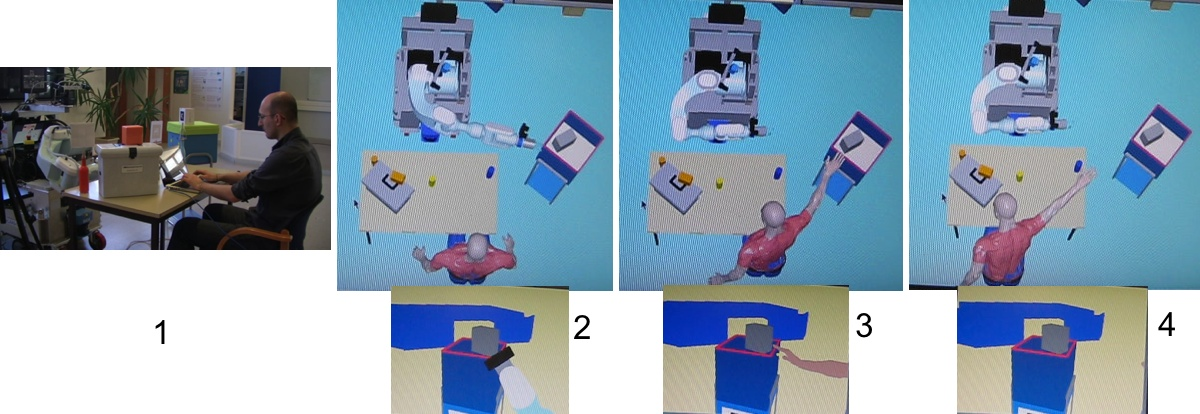
\includegraphics[width=1.0\textwidth]{figs/reachex.jpg}	
	\caption{An example illustrating the \textit{reachable} relation. The relation is computed from the perspectives of both the robot and the human. The computed posture at each step is illustrated with a global view of the scene (top), and from a closest view (bottom).}
\label{fig::reach-ex}
\end{figure*}

\begin{figure}[ht!]
   \label{fig:sparkSubfigures}
   \begin{center}
%
       \subfigure[Initial state]{%
%           \label{fig:wuweiPhoto}
           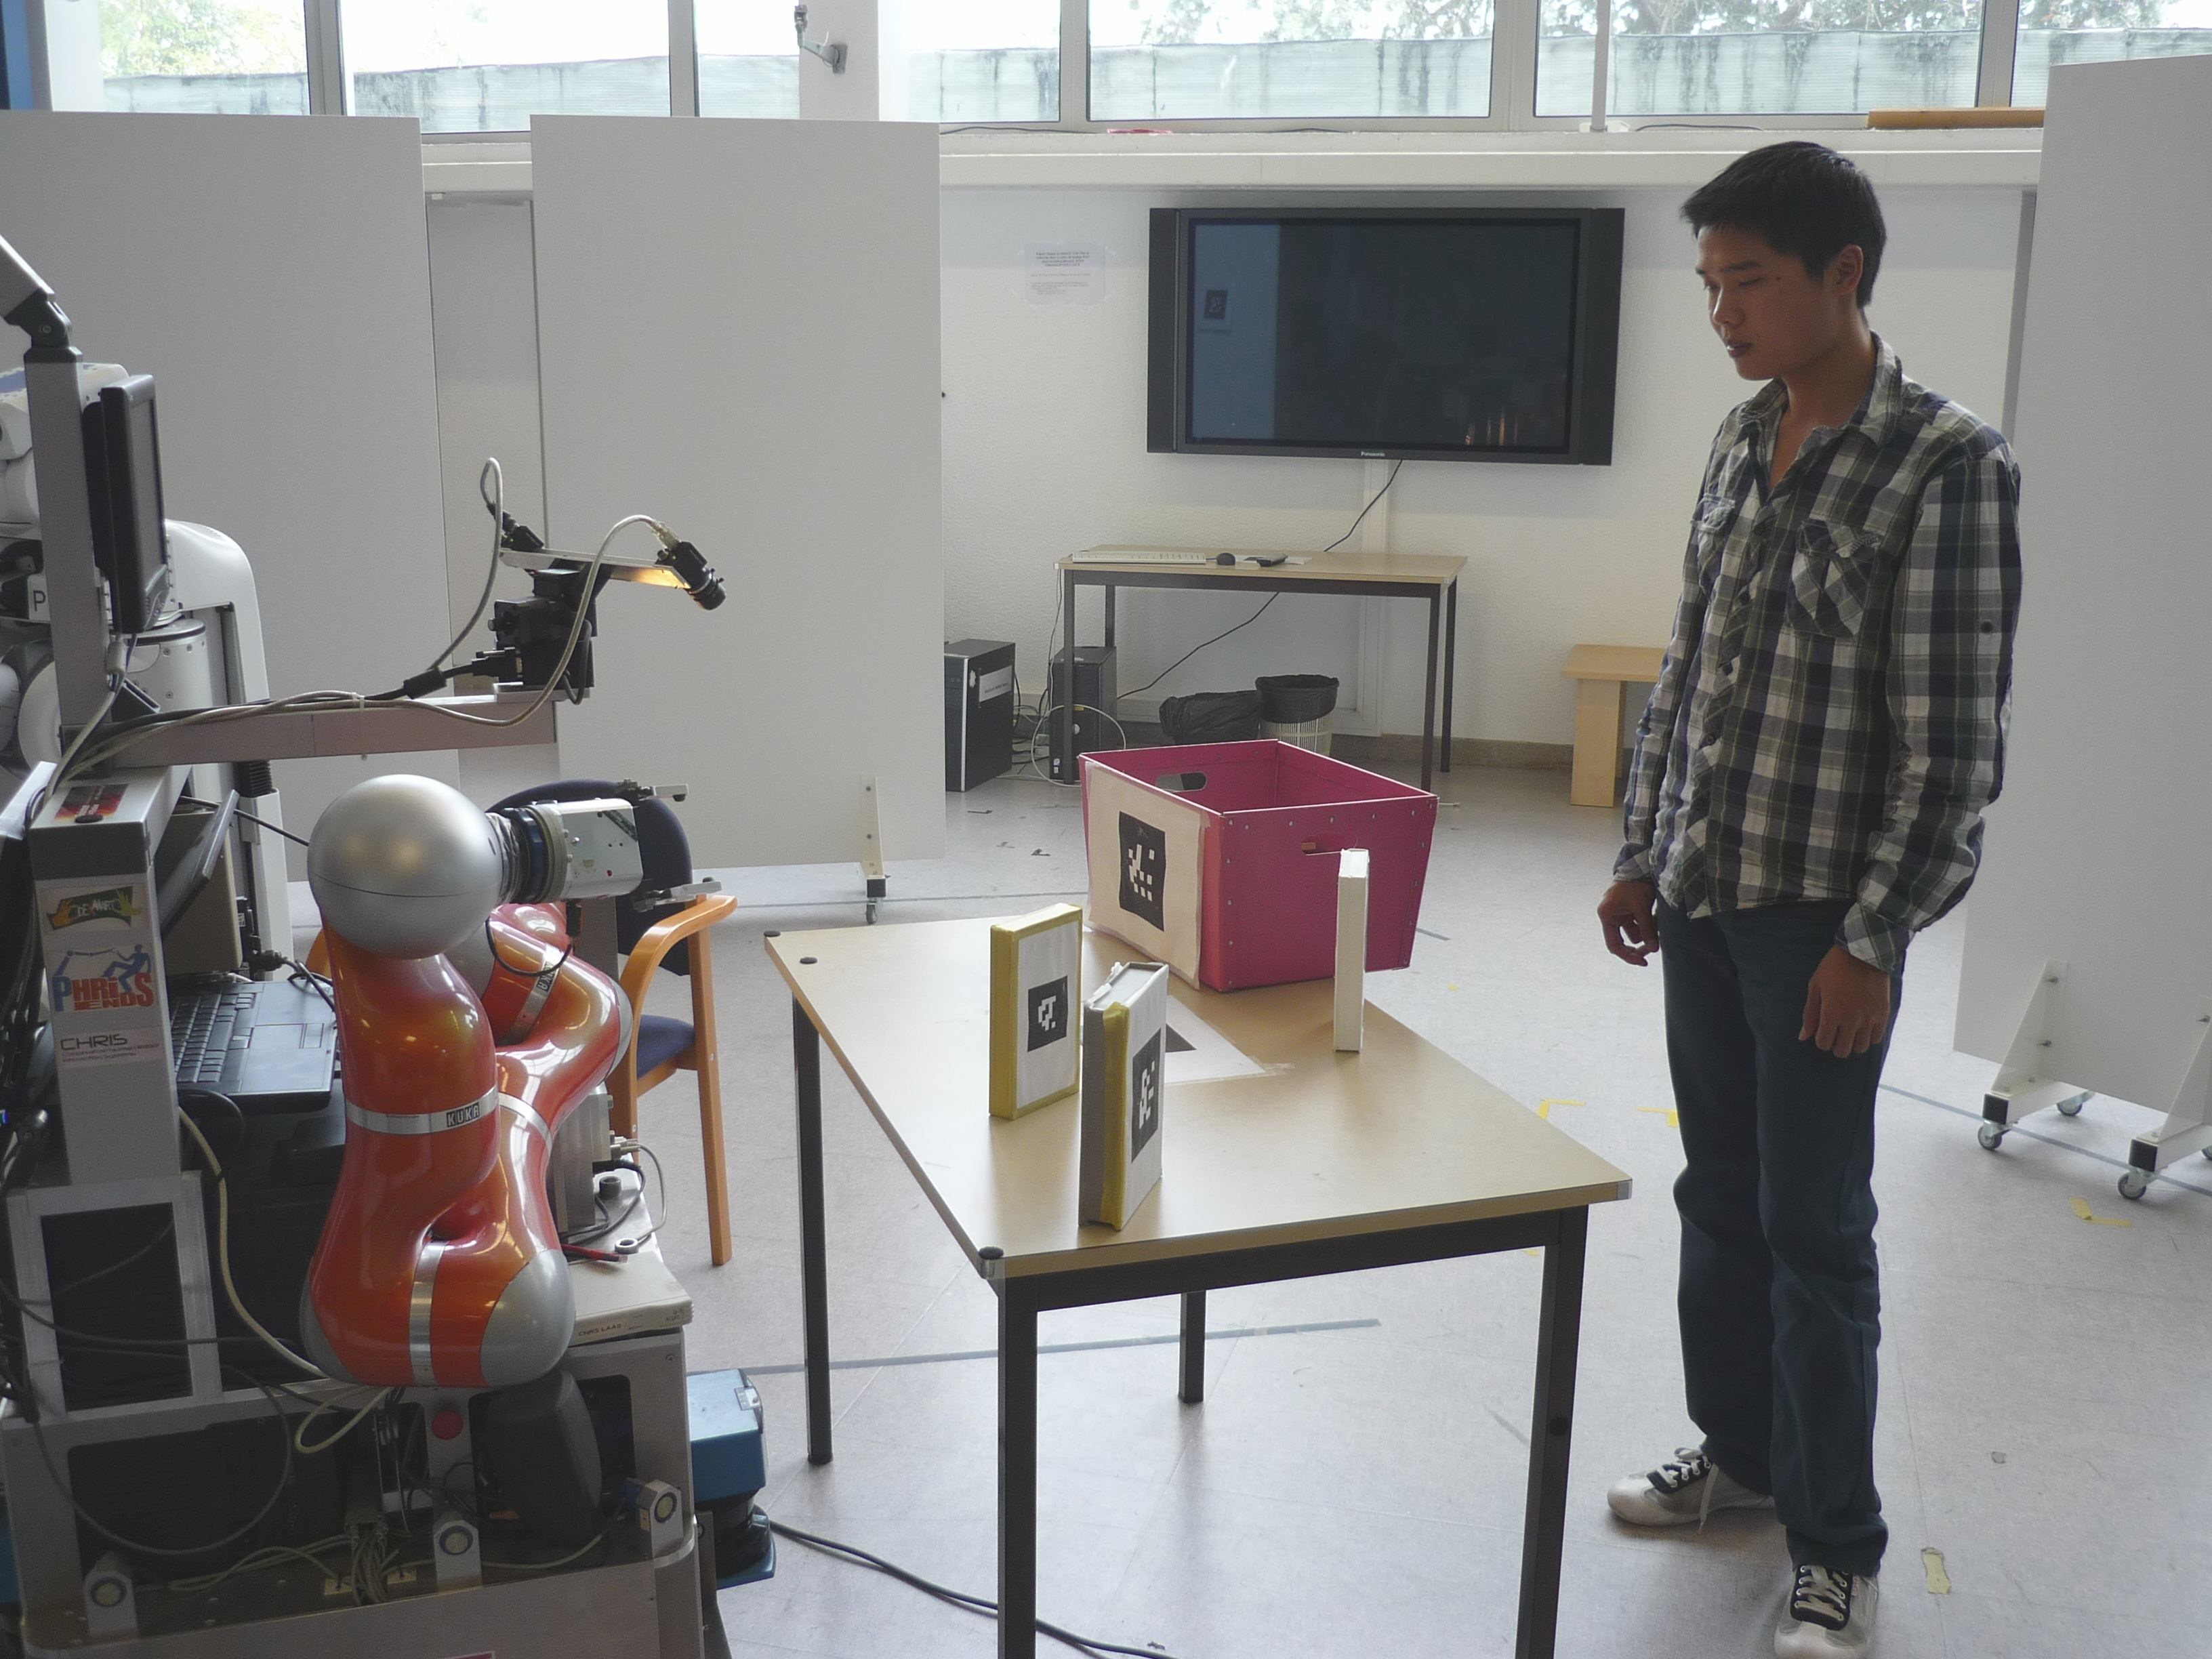
\includegraphics[width=0.5\textwidth]{./figs/etat2-P1010769_brightened-v2.jpg}
       }%
       \subfigure[3d model view of initial state]{%
%          \label{fig:sparkScreenshot}
          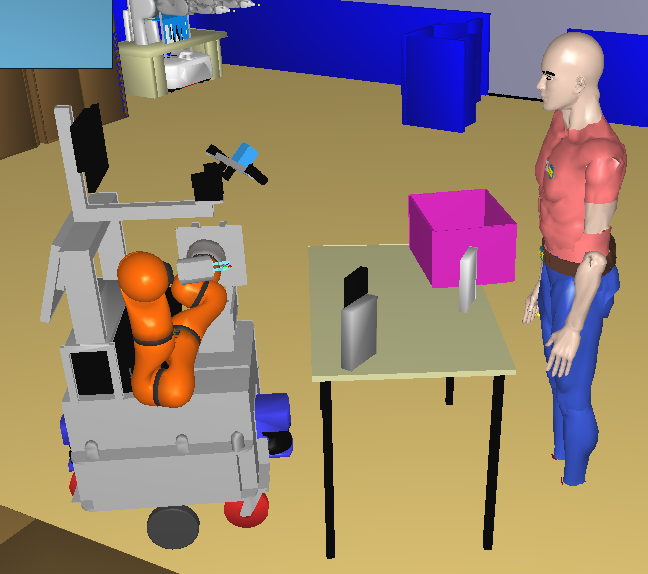
\includegraphics[width=0.43\textwidth]{./figs/etat2_photo.png}
       }\\ %  ------- End of the first row ----------------------%
%
   \end{center}

   \caption{%
     In this situation, there are three tapes on the table. Two tapes
     are only reachable by the robot: the LOTR\_TAPE (black in the 3d
     model) and GREY\_TAPE. The third tape WALLE\_TAPE (white in the
     3d model) and the trashbin PINK\_TRASHBIN are only reachable by
     the human HUMAN1. All tapes are on the table TABLE.  }%

\end{figure}

The set of facts computed in the situation depicted by
Figure~\ref{fig:sparkSubfigures} is the following:
\begin{footnotesize}
%\begin{small}
\begin{verbatim}
                ROBOT                          HUMAN1
PINK_TRASHBIN isReachable false    PINK_TRASHBIN isReachable true 
WALLE_TAPE isReachable false       WALLE_TAPE isVisible true 
LOTR_TAPE isReachable true         LOTR_TAPE isReachable false 
GREY_TAPE isReachable true         GREY_TAPE isReachable false
WALLE_TAPE isVisible true          WALLE_TAPE isReachable true 
LOTR_TAPE isVisible true           LOTR_TAPE isVisible true 
GREY_TAPE isVisible true           GREY_TAPE isVisible true 
WALLE_TAPE isOn TABLE              WALLE_TAPE isOn TABLE 
LOTR_TAPE isOn TABLE               LOTR_TAPE isOn TABLE 
GREY_TAPE isOn TABLE               GREY_TAPE isOn TABLE 
\end{verbatim}
%\end{small}
\end{footnotesize}

%\newline\newline
%\subsubsection*{Hypotheses on objects states and positions}
\vspace{0.3cm}
\noindent
\textbf{Hypotheses on objects states and positions:}
It is sometimes difficult or even impossible to see and/or track an
object in certain states. This happens, for instance, when the object
has been put in a container, when it is in the robot gripper or in the
human hand, and more generally in any state in which it is hidden by
something else. Our robot has a model of the possible symbolic states
for an object (whether the object is on a furniture, in an agent hand,
in a container, etc.).  According to the robot perception of what has
happened since the object was last seen, the robot tries to maintain a
belief of the current possible symbolic states and their associated
probabilities for this object. Such information can be used to update
the beliefs using input from exploration, dialog, human visual
focus,\ldots
SPARK currently provides a simple implementation of such a functionality. The
only managed hypotheses are \emph{in container} and \emph{in agent hand}. We
can have only one hypothesis at the same time. Hypothesis validity is checked
geometrically in case of incoming perception values.


%\subsubsection*{Primitive action recognition}
\vspace{0.3cm}
\noindent {\bf Primitive action recognition:} 
Monitoring human activity is crucial to maintain a coherent state of
the world. Full human action and activity monitoring is a difficult
task that requires knowledge and reasoning both on high level facts
like goals, intentions and plans, as well as bottom-up data from agent
and object motions. Simple temporal and geometric reasoning on human
hand trajectories and potential objects placements can provide some
useful clues for high level human monitoring processes. We call this
temporal and geometric reasoning \emph{primitive action recognition}.

For example, a \emph{pick}, a \emph{throw} or a \emph{place} action
can be recognized by observing that an object on table and an empty
human hand are close to each other, or that the human hand holding an
object is close to a container, etc. Human hand position is either
directly perceived or inferred from its initial perceived trajectory.
We have a simple implementation of such a primitive action recognition
in SPARK that relies on monitoring human hand and its motion near
objects or above containers.

\subsection{Symbolic facts and beliefs management}

The facts produced by the geometric and temporal reasoning component
are stored in a central symbolic knowledge base, called ORO. Besides
acting as a facts database, the ORO platform~\cite{Lemaignan2010}
exposes several functions: operations on knowledge statements relying
on inference (through a continuous first-order logic classification
process), management of \emph{per-agent} symbolic models, and also
higher cognitive and human-robot interaction related functionalities
like categorization of sets of concepts, profiles of memory (that
enable the robot to ``forget'' about some facts), natural language
grounding~\cite{Lemaignan2011}\ldots.

ORO stores independent knowledge models (in our implementation, as
\emph{ontologies}) for each agent (the robot and the humans it
interacts with). The robot architecture components (like the executive
layer or the situation assessment component) can then store the
agents' beliefs in specific models.  Each of these models is
independent and logically consistent, enabling reasoning on different
perspectives of the world that would otherwise be considered as
globally inconsistent (for instance, an object can be visible for the
robot but not for the human. This object can have at the same time the
property \concept{isVisible \textbf{true}} and \concept{isVisible
  \textbf{false}} in two different models). This feature actually
allows us to consider the robot to be endowed with a simple
\emph{theory of mind}~\cite{Scassellati2002}: it can explicitly
model the belief state of its interactors.

ORO also provides an event mechanism that allows components to be
triggered when specific events occur. A component can
for instance subscribe to events of kind \setstmt{?agent isVisible
  true, ?agent type Human}. As soon as the perception layer detects a
human in the robot's field of view and accordingly updates the
knowledge base, the executive layer would be triggered back. The
event framework also takes advantage of the inference capabilities of
ORO. Thus an event can be indirectly triggered if its triggering
conditions can be inferred to be true.

\subsection{Situation Assessment and Context Management Controller} 

Building, updating and maintaining a correct state of the world at
geometric and symbolic level is crucial to the capacity of the robot
to carry on successfully a multi-step interaction with a human. Tight
integration between the robot controller and the geometric and
temporal reasoning functions in SPARK and symbolic facts and beliefs
management in ORO is central.
 
The robot controller has access to the symbolic facts in ORO that are
automatically updated whenever object and agent positions are changed.
Robot controller can also access geometric perceived or inferred
positions of objects and geometric positions and postures of the human
that will be used to orient its cameras.  Building and updating the
state of the world first relies on perceiving objects. Robot
controller can use:

\begin {itemize}
\item Exploration policies: robot will exhaustively scan the table to
  see all what can be seen.

\item Search policies: robot will search an object until it is
  detected if possible, scanning all the table and looking in human
  hand.

\end {itemize} 

Robot reasons on possible positions for non perceived
objects. These hypotheses could be updated using new input from dialogue, human
action and focus of attention. Currently, we manage at most one hypothesis per
object. This hypothesis is produced by robot controller through an inference on
robot or human action. In case of perception conflicts with low probability for
the current hypothesis, robot controller will break this hypothesis and delete
corresponding symbolic fact in the ontology.

Robot must reacts to change in the world not linked to robot
action to drive world update. Robot controller uses SPARK to monitor human hand
motion and primitive action recognition for \emph{pick} and \emph{throw}. As
mentioned above these primitive action recognition should be used with higher
level information on goals, intentions and plans and some exploration to
achieve complex human action and activity monitoring.  In the current
implementation, these primitive actions are over-optimistically interpreted as
the corresponding actions \emph{pick} object and \emph{throw} object.

\section{Goal and Plan Management}\label{sec:plan}

The Goal and Plan Management activity involves the human-aware
symbolic task planner component and the dedicated robot controller
activity (Figure~\ref{architecture_fg}).

\subsection{Symbolic Task Planning}

In order to devise how a given goal can be accomplished, the robot has
to elaborate a plan,~\textit{i.e.} a set of actions to be achieved by
the robot and its human partners.  This is the role of a HATP
\cite{Alili2008} (for Human Aware Task Planner).  HATP is based on a
Hierarchical Task Network (HTN) refinement which performs an iterative
task decomposition into sub-tasks until reaching atomic
actions~\cite{Nau2003}.  The planning domain defines a set of methods
describing how to decompose a task and can be seen as the Howto
knowledge of the robot.  HATP is able to produce plans for the robot's
actions as well as for the other participants (humans or robots). It
can be tuned by setting up different costs depending on the actions to
apply and by taking into account a set of constraints called social
rules. This tuning aims at adapting the robot's behavior according to
the desired level of cooperation of the robot.

%\subsubsection*{Agents and action streams:}
\vspace{0.3cm}
\noindent
\textbf{Agents and action streams:}
The robot plans not only for itself but also for the other agents. The
resulting plan, called ``shared plan'' is a set of actions that form
a stream for each agent involved in the goal achievement. Depending on
the context, some ``shared plans'' contain causal relations between
agents. For example, the second agent needs to wait for the success of
the first agent's action to be able to start its own action. When the
plan is performed, causal links induce synchronization between
agents. Figure~\ref{plan_hatp1} illustrates a plan with two streams.

\begin{figure}[htbp]
  \centering
  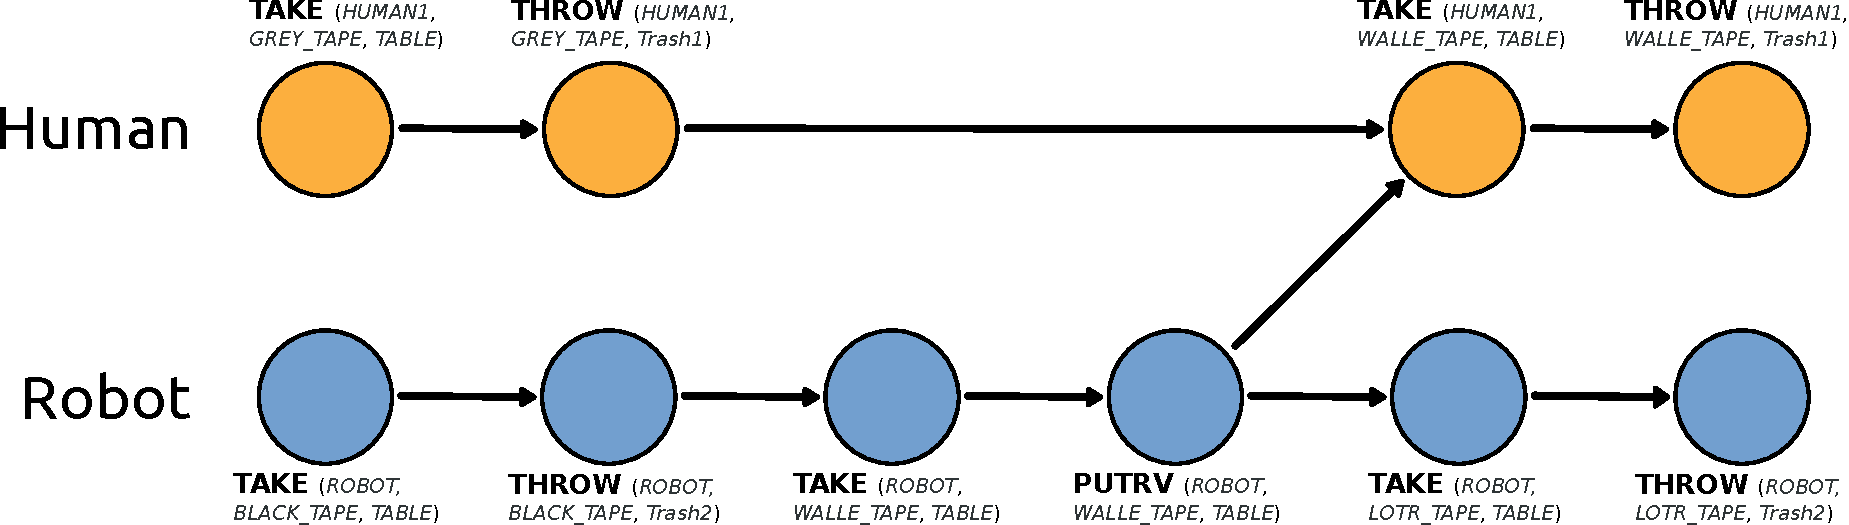
\includegraphics[width=0.95\columnwidth]{./figs/first_plan.pdf}
  \caption{A plan produced by HATP with 2 streams}
  \label{plan_hatp1}
\end{figure}

%\subsubsection*{Action costs and social rules:}
\vspace{0.3cm}
\noindent
\textbf{Action costs and social rules:}
A cost and a duration function is associated to each action.
The duration function provides a duration interval for the action
achievement and is used, in one hand, to schedule the different
streams and, in the other hand, as an additional cost function.
In addition to these costs, HATP also takes into account a set of social
rules.  Social rules are constraints aiming at leading the plan
construction towards the best plan according to some human
preferences. The social rules we have defined so far deal with:

\begin{itemize}
\item undesirable state: to avoid a state in which the human could
  feel uncomfortable;
\item undesirable sequence: to eliminate sequences of actions that can
  be misinterpreted by the human;
\item effort balancing: to adjust the work effort of the agents;
\item wasted time: used to avoid long delays between the actions of
  the human partner;
\item intricate links: to limit dependencies between the actions of
  two or more agents.
\end{itemize}

\begin{figure}[htbp]
  \centering
  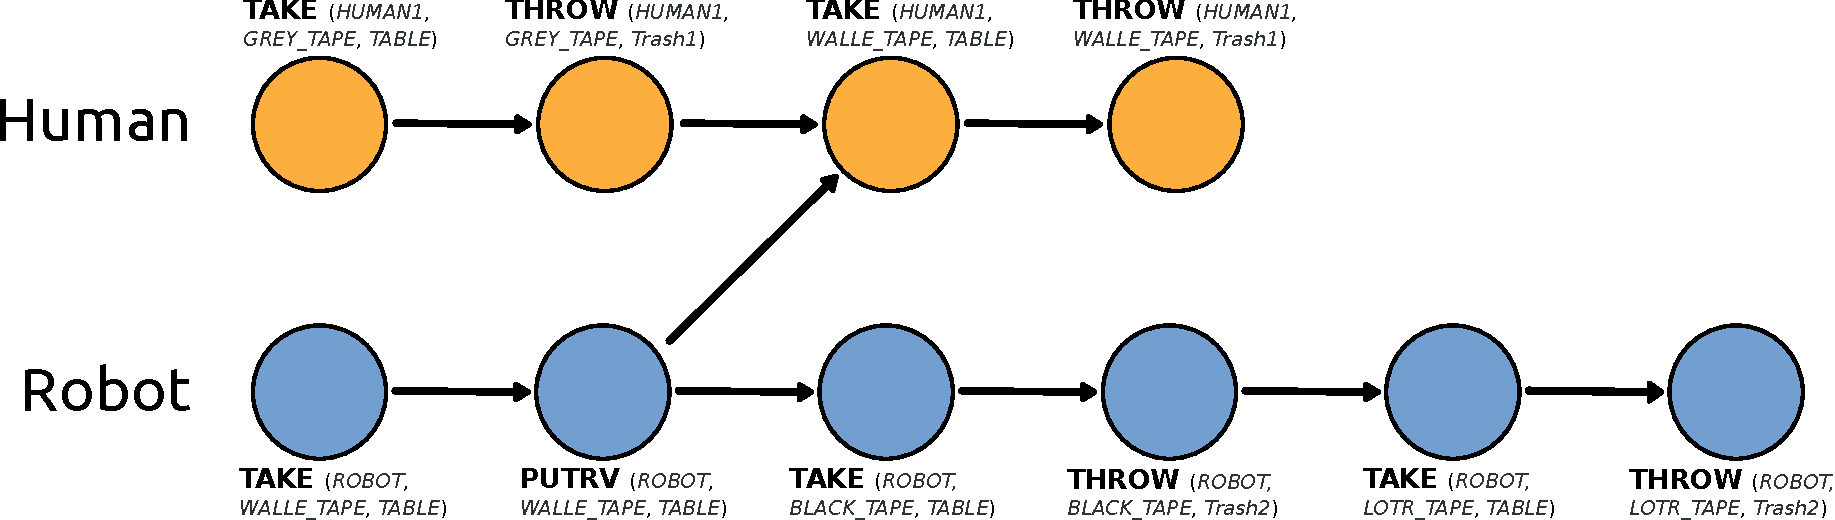
\includegraphics[width=0.95\columnwidth]{./figs/second_plan.pdf}
  \caption{A plan with the wasted time social rule}
  \label{plan_hatp2}
\end{figure}

Figure~\ref{plan_hatp2} illustrates an alternative plan to the previous 
one (Figure~\ref{plan_hatp1}) if the wasted time social rule is used.
The obtained shared plan is the best plan according to a global evaluation of
these multiple criteria.

%\subsubsection*{Several levels of cooperation:} 
\vspace{0.3cm}
\noindent
\textbf{Several levels of cooperation:} 
By tuning its costs
and adapting its social rules, HATP can be used to compute various
alternative plans. These plans can be categorized into several levels
of cooperation

\begin{itemize}
\item helping the human to achieve his goal by acting for him
\item sharing concrete resources by handing some objects
\item collaboration of the robot and the human by coordinating their
  actions towards a human-robot joint goal.
\end{itemize}

\subsection{ Goal and plan Controller}
Figure~\ref{goal_plans_fg} sums up the Goal and Plan Management as
implemented in the robot controller.  When an event announcing a new
goal is caught by the controller, the validity of this goal is tested:
does it corresponds to capabilities of agents? is it not already
achieved? Then, the goal is sent to HATP which produces a first plan.
A goal is considered achievable as long as the planner computes a
valid plan and it is not abandoned by the human.

Plan execution consists in the management of all the actions of the
plan. Human and robot are not acting both at the same time.  In case
of plan failure a new plan is requested and executed.

The management at the action level is done in three steps. First, the
action preconditions are tested over the current state of the
world. Then the action is executed and monitored (only monitored of it
corresponds to a human action).  Finally, the expected effects are
verified in order to acknowledge the action achievement.

Concerning the speech acts during plan management, the robot informs
its partners on the goal existence and status, plan existence and
status, ongoing plan action, plan action failure, failing facts for
action precondition or effect assessment.

\begin{figure}[thpb]
  \centering
  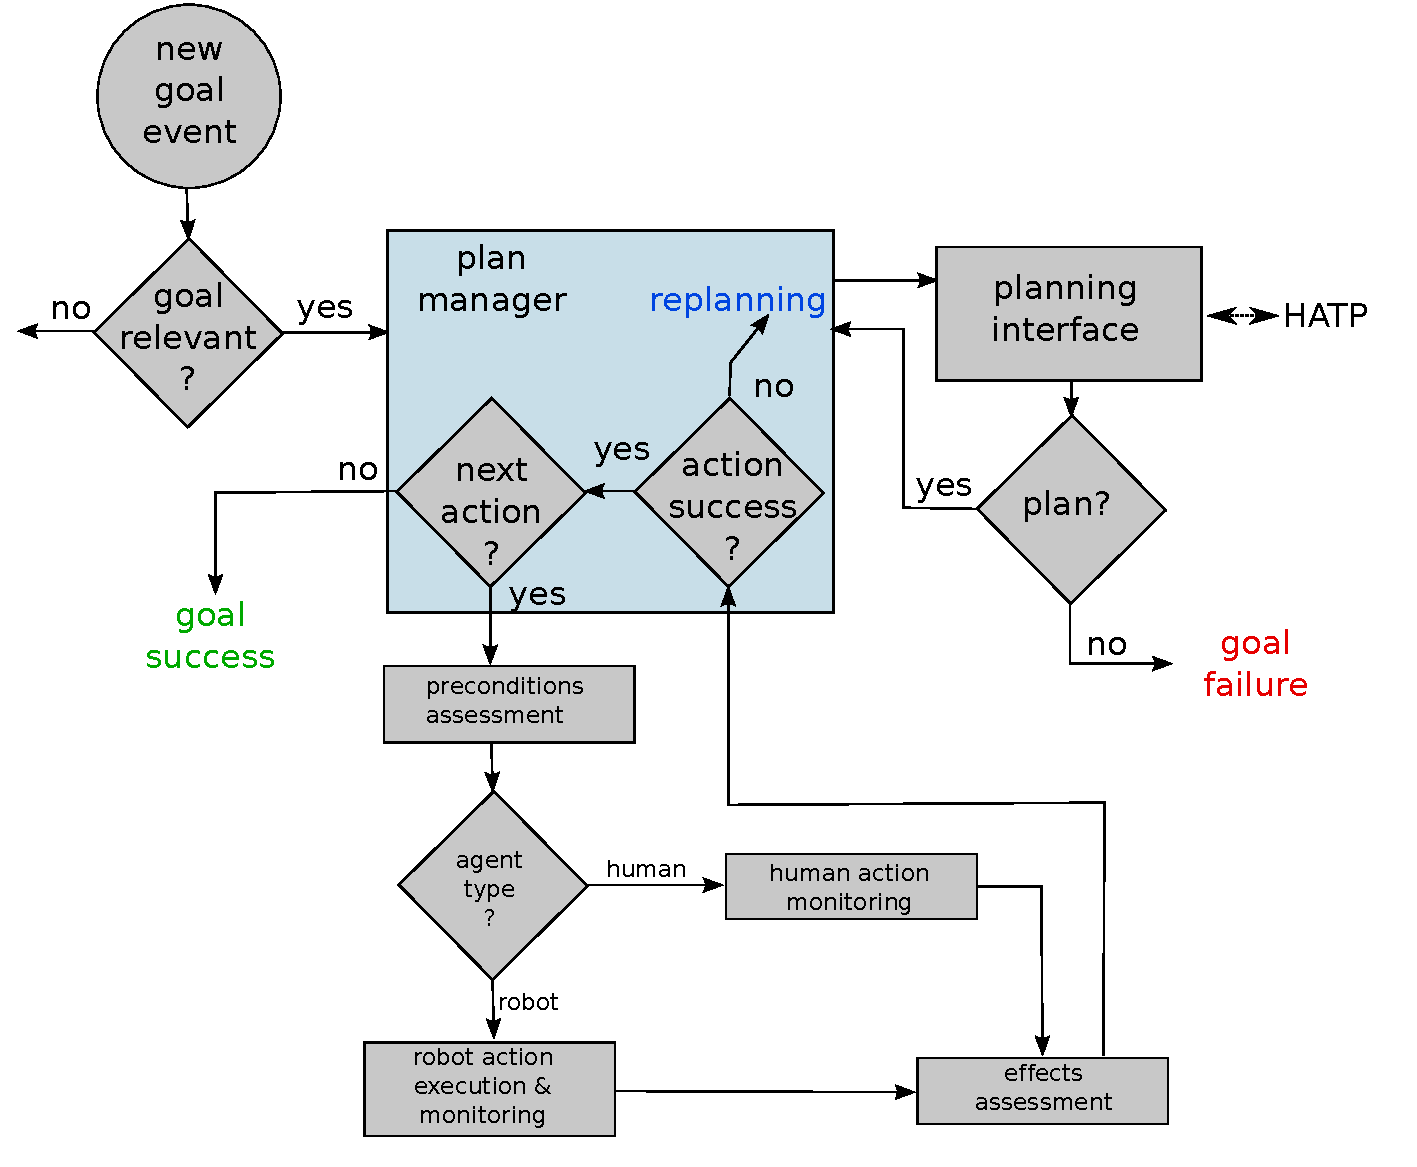
\includegraphics[width=0.8\columnwidth]{./figs/plan_management.pdf}
  \caption {Automaton for goal and plan management}
  \label{goal_plans_fg}
\end{figure}



\section{Action execution and monitoring}\label{sec:action}

The action execution and monitoring task involves the motion and task
planning, the effectors and the dedicated robot controller activity
(Figure~\ref{architecture_fg}).


%\subsubsection*{Human aware motion, placement and manipulation planning}
\vspace{0.3cm}
\noindent
\textbf{Human-aware motion, placement and manipulation planning:}
In our scenarios, actions are only object manipulation actions: Pick,
Place, Throw, Give. Motion and Task planning allows to compute final
object placement, grasp and arm motion trajectories taking into
account task specific constraints and human postures, abilities and
preferences: see \cite{Sisbot2008, Mainprice2011, Pandey2010} for
details.


%\subsubsection*{Action Execution and Monitoring Robot Controller}
\vspace{0.3cm}
\noindent
\textbf{Execution and Monitoring Robot Controller:} Depending on the
context and on the shared plan elaborated by HATP for a given goal,
the robot controller decides to execute an action or to ask its human
partner to do it.  Actions feasibility by the human or the robot are
regularly reconsidered based on the reachability / visibility
computation mechanisms.

Robot action execution is based on simple automatons  that translate
symbolic planning atomic actions into sequences of planned arm motions
and gripper commands to execute according to current state
of the 3-tuple (gripper, object, furniture). We have three states
according to whether the object is in gripper and if it is in gripper
whether it is on furniture.  These states are directly obtained from
the updated symbolic state of the world in the ontology.

For plan action monitoring, primitive actions recognition defined
above are used. A primitive action detection is interpreted as action
success if it is the expected one and failure otherwise. The robot
also reacts to the absence of activity.

\section{An illustrative example}\label{sec:expes}

We assume here that the robot (and the human) has been given the joint goal
``CLEAN TABLE''. For HATP, this means putting all tapes that are
currently on the table in the trashbin. Depending on the state of the
world and agent preferences, different plans are produced.

Figure~\ref{plan-etat2} shows a plan produced to clean the table based on the initial the initial state given in  \S~\ref{sub:gtrc}.

\begin{figure*}[thpb]
  \centering
  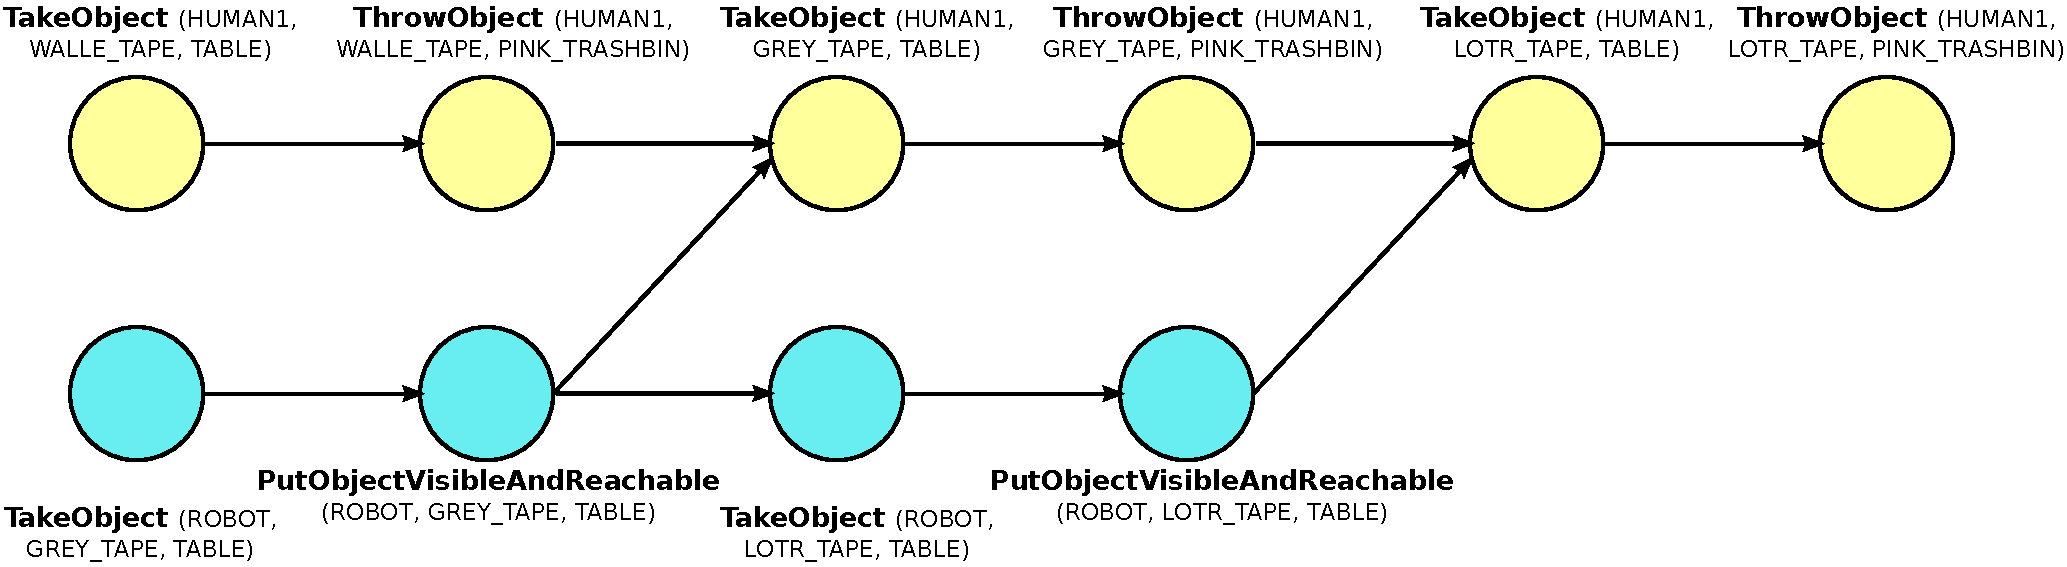
\includegraphics[width=1.0\textwidth]{./figs/plan3.pdf} \\
  \caption {A plan produced by HATP for clean the table based on the initial state given in \S~\ref{sub:gtrc}}
  \label{plan-etat2}
\end{figure*}

Let us now take a simpler example to illustrate a full run of the
system. We have only one tape on the table and it is is reachable only
by the robot while the throw position on top of the trashbin is
reachable only by the human.

\begin{figure*}[thpb]
  \centering
    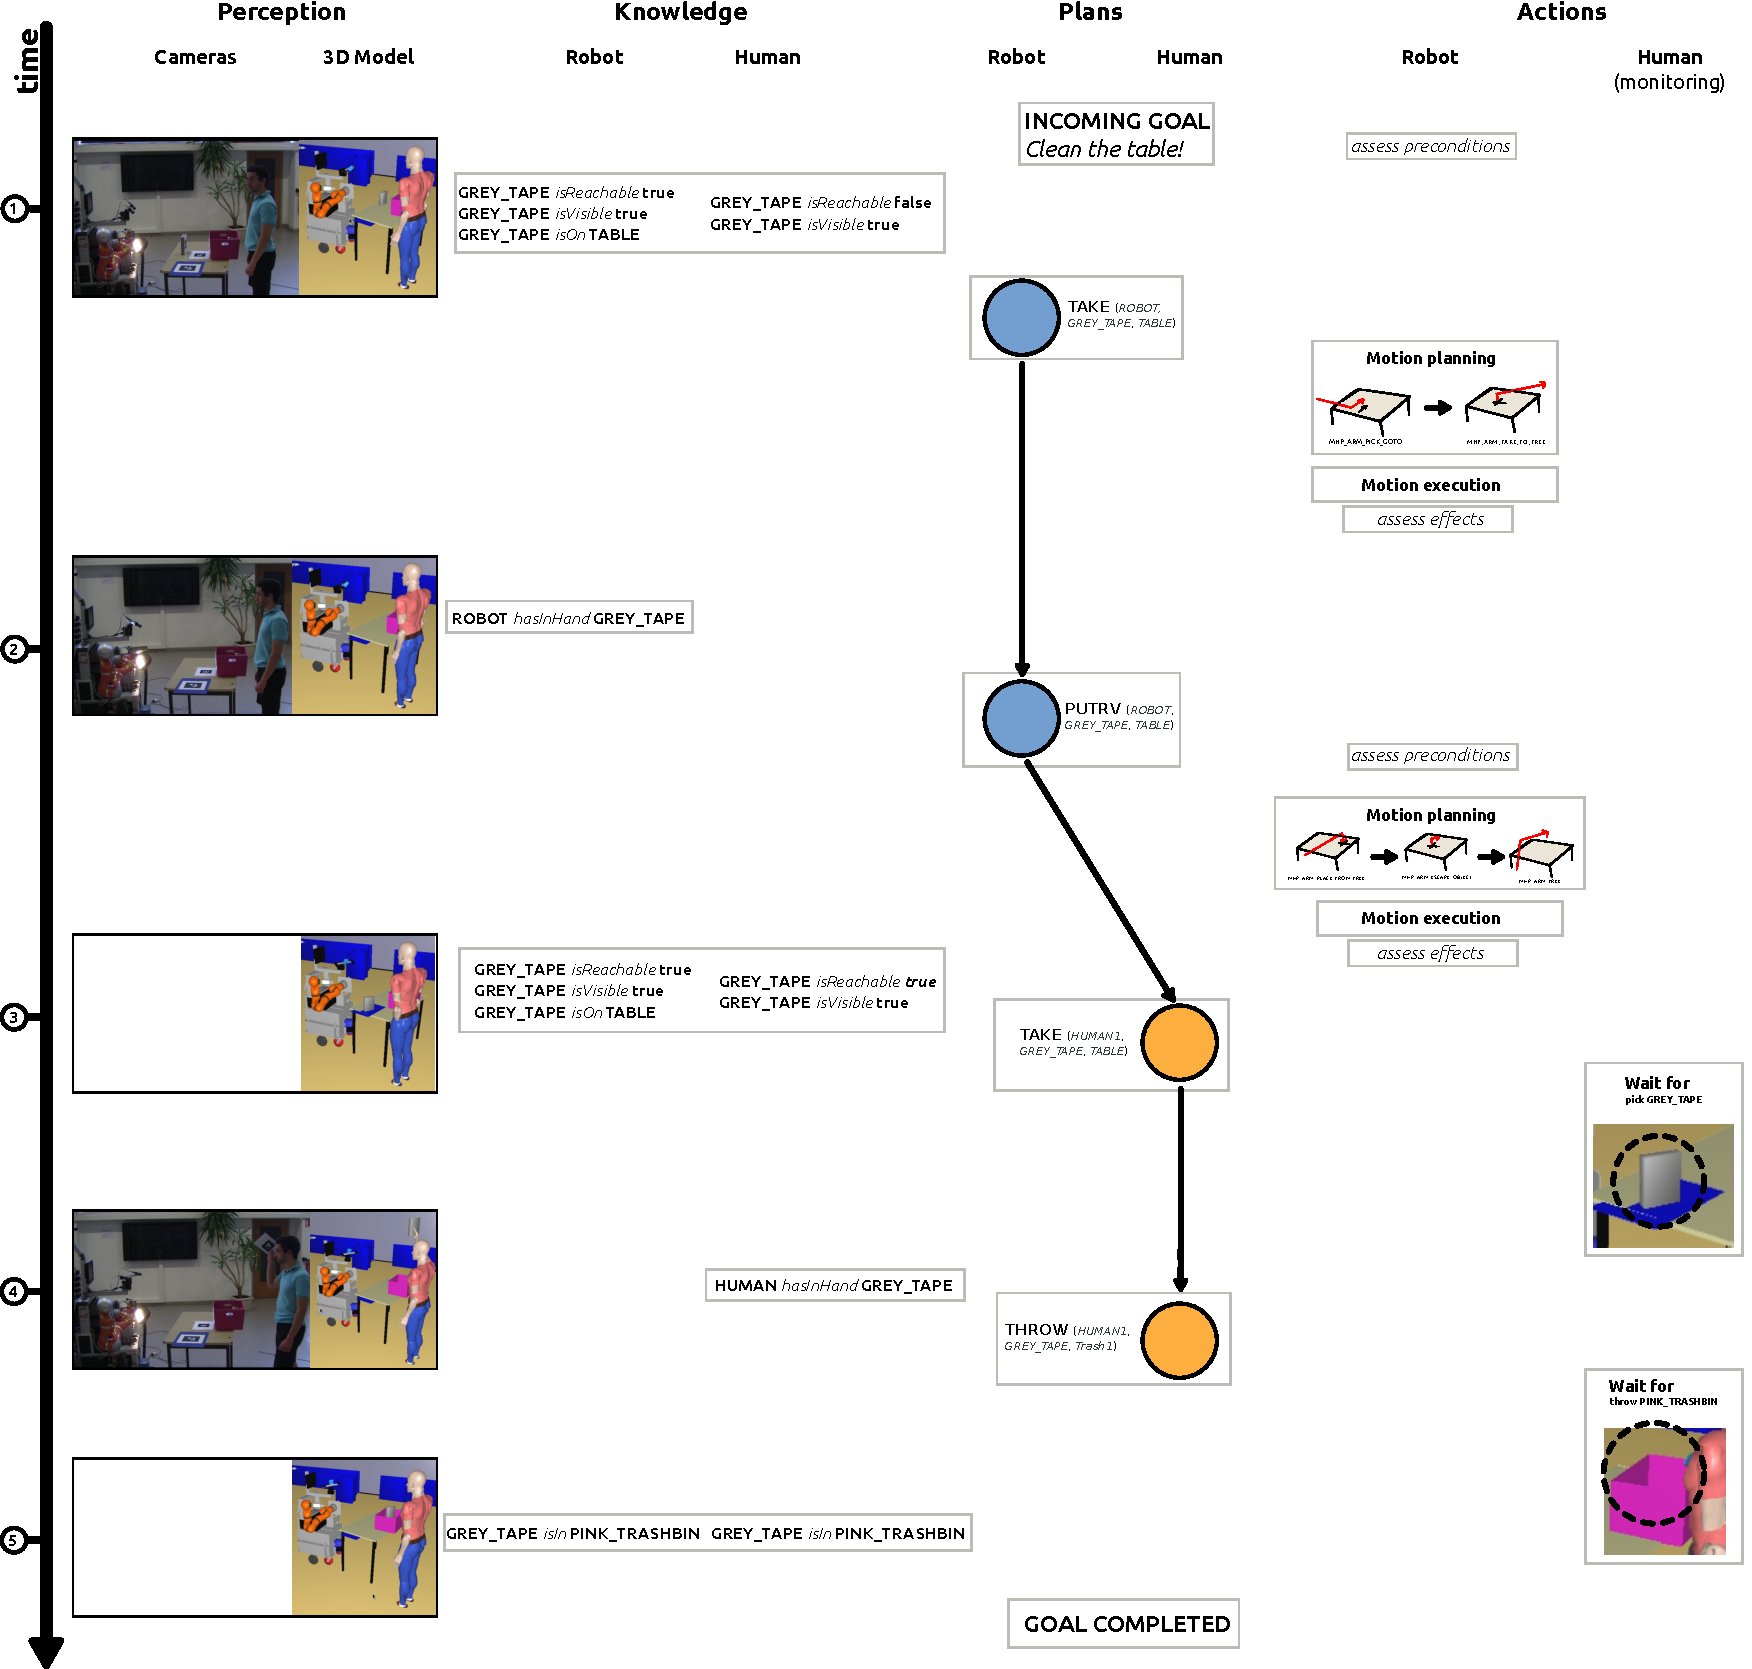
\includegraphics[width=1.0\textwidth]{./figs/manip_run.pdf} \\
    \begin{center}
    \caption {An example of a human-robot collaborative goal achievement}
    \end{center}
  \label{manip_run_fg}
\end{figure*}


%\subsection{successful execution}

Figure~\ref{manip_run_fg} illustrates the main processes occurring
during a multi-step human-robot collaborative goal achievement.  The
plan produced is quite straightforward and is shown in the third row
called ``Goal and Plan''. It consists in 4 successive actions
involving the robot and the human. Robot grasps the tape and then
places it on the table at a position where it is visible and reachable
for the human. Human then is asked to pick the tape and throw it in
the trashbin. The first row, named ``Cameras'', shows several
snapshots corresponding to various execution steps. Snapshot~1
presents the initial situation. Snapshots~2, 3, 4 and 5 give the state
after the successive achievement of the four actions in the plan. The
second row, named ``3D Model'', shows the display of SPARK at the same
instants. The fourth, row called ``Robot Speech Acts'', gives robot
speech acts produced along the execution to inform the human partner
about goal and plan creation and status and to verbalize the actions
that the human is asked to execute. The fifth row illustrates robot
knowledge on itself and on the objects. The sixth row illustrates the
robot knowledge about the human state. The seventh row gives ongoing
robot action with action preconditions and effects assessment as well
as motion execution tasks. Motion trajectory typology can be found
between the 3D Model views. The eighth row gives ongoing human action
with action preconditions and effects assessment and monitoring
activity.

\section{Conclusion and future work}

In this paper we have presented a decisional framework designed for
robots operating in a human environment. Our objective is to provide a
management of human-robot interaction that is an integral part of a
general robot control architecture.  This was done in order to provide
a principled way to deal with HRI scenario.  The framework is also
suitable for the development and experiment of task planners and
interaction schemes that explicitly consider human abilities and
preferences.

The design choices and the results presented here are still preliminary.
While the general scheme we propose might be difficult to implement in
a general sense, we believe that it is a reasonable challenge to
implement it in the case of a personal robot assistant essentially
devoted to fetch-and-carry, as well as for interactive manipulation
tasks and associated activities.\\

\vspace{0.3cm}
\noindent
{\bf Acknowledgements:}
This work has been conducted within the EU CHRIS project ({\tt
  \url{http://www.chrisfp7.eu/}}) funded by the E.C. Division FP7-IST
under Contract 215805. We also would like to thank warmly a number of LAAS
robotics team members and more particularly Xavier Broquere, Mokhtar
Gharbi, Wuwei He, Matthieu Herrb, Jim Mainprice, Raquel Ros, Daniel
Sidobre, Thierry Sim\'{e}on, Muhammad Ali.

%%%%%%%%%%%%%%%%%%%%%%%%%%%%%%%%%%%%%%%%%%%%%%%%%%%%%%%%%%%%%%%%%%%%%%%%%%%%%%%%
\bibliographystyle{elsarticle-num}
\bibliography{laas_hri}



\end{document}





\section{Discussion and future work}

The design choices and the results presented here is still preliminary. 
While the general scheme we propose might be difficult to implement in
a general sense, we believe that it is a reasonable challenge to
implement it in the case of a personal robot assistant essentially
devoted to fetch-and-carry, as well interactive manipulation tasks and
associated activities. The robot would operates in a known in-door
environment (acquired in a preliminary phase).

In such contexts, it is possible ....



Fetch-and-carry and object manipulation task need 3D geometric
planning.  One challenging problem would be to extend the approach
discussed above to the situation where a robot has to hand
an object to human. Indeed, there is a need to take into account
visibility and reach, in terms of kinematic constraints, of the human
partner (Figure~\ref{fig_handing}).


%\input{conclusion} %% Conclusion and Future Work
\section{Conclusion}\label{sec:Conclusion}

In this paper we have presented a decisional framework designed for
robots operating in a human environment. Our objective is to provide a
management of human interaction that is an integral part of a general
robot control architecture.  This was done in order to provide a
principled way to deal with HRI.

The framework is also suitable for the development and experiment of
task planners and interaction schemes that explicitly consider
human abilities and preferences.

Examples of such planners are presented that integrate various models
of human abilities and preferences.


\end{document}

